\documentclass[1p]{elsarticle_modified}
%\bibliographystyle{elsarticle-num}

%\usepackage[colorlinks]{hyperref}
%\usepackage{abbrmath_seonhwa} %\Abb, \Ascr, \Acal ,\Abf, \Afrak
\usepackage{amsfonts}
\usepackage{amssymb}
\usepackage{amsmath}
\usepackage{amsthm}
\usepackage{scalefnt}
\usepackage{amsbsy}
\usepackage{kotex}
\usepackage{caption}
\usepackage{subfig}
\usepackage{color}
\usepackage{graphicx}
\usepackage{xcolor} %% white, black, red, green, blue, cyan, magenta, yellow
\usepackage{float}
\usepackage{setspace}
\usepackage{hyperref}

\usepackage{tikz}
\usetikzlibrary{arrows}

\usepackage{multirow}
\usepackage{array} % fixed length table
\usepackage{hhline}

%%%%%%%%%%%%%%%%%%%%%
\makeatletter
\renewcommand*\env@matrix[1][\arraystretch]{%
	\edef\arraystretch{#1}%
	\hskip -\arraycolsep
	\let\@ifnextchar\new@ifnextchar
	\array{*\c@MaxMatrixCols c}}
\makeatother %https://tex.stackexchange.com/questions/14071/how-can-i-increase-the-line-spacing-in-a-matrix
%%%%%%%%%%%%%%%

\usepackage[normalem]{ulem}

\newcommand{\msout}[1]{\ifmmode\text{\sout{\ensuremath{#1}}}\else\sout{#1}\fi}
%SOURCE: \msout is \stkout macro in https://tex.stackexchange.com/questions/20609/strikeout-in-math-mode

\newcommand{\cancel}[1]{
	\ifmmode
	{\color{red}\msout{#1}}
	\else
	{\color{red}\sout{#1}}
	\fi
}

\newcommand{\add}[1]{
	{\color{blue}\uwave{#1}}
}

\newcommand{\replace}[2]{
	\ifmmode
	{\color{red}\msout{#1}}{\color{blue}\uwave{#2}}
	\else
	{\color{red}\sout{#1}}{\color{blue}\uwave{#2}}
	\fi
}

\newcommand{\Sol}{\mathcal{S}} %segment
\newcommand{\D}{D} %diagram
\newcommand{\A}{\mathcal{A}} %arc


%%%%%%%%%%%%%%%%%%%%%%%%%%%%%5 test

\def\sl{\operatorname{\textup{SL}}(2,\Cbb)}
\def\psl{\operatorname{\textup{PSL}}(2,\Cbb)}
\def\quan{\mkern 1mu \triangleright \mkern 1mu}

\theoremstyle{definition}
\newtheorem{thm}{Theorem}[section]
\newtheorem{prop}[thm]{Proposition}
\newtheorem{lem}[thm]{Lemma}
\newtheorem{ques}[thm]{Question}
\newtheorem{cor}[thm]{Corollary}
\newtheorem{defn}[thm]{Definition}
\newtheorem{exam}[thm]{Example}
\newtheorem{rmk}[thm]{Remark}
\newtheorem{alg}[thm]{Algorithm}

\newcommand{\I}{\sqrt{-1}}
\begin{document}

%\begin{frontmatter}
%
%\title{Boundary parabolic representations of knots up to 8 crossings}
%
%%% Group authors per affiliation:
%\author{Yunhi Cho} 
%\address{Department of Mathematics, University of Seoul, Seoul, Korea}
%\ead{yhcho@uos.ac.kr}
%
%
%\author{Seonhwa Kim} %\fnref{s_kim}}
%\address{Center for Geometry and Physics, Institute for Basic Science, Pohang, 37673, Korea}
%\ead{ryeona17@ibs.re.kr}
%
%\author{Hyuk Kim}
%\address{Department of Mathematical Sciences, Seoul National University, Seoul 08826, Korea}
%\ead{hyukkim@snu.ac.kr}
%
%\author{Seokbeom Yoon}
%\address{Department of Mathematical Sciences, Seoul National University, Seoul, 08826,  Korea}
%\ead{sbyoon15@snu.ac.kr}
%
%\begin{abstract}
%We find all boundary parabolic representation of knots up to 8 crossings.
%
%\end{abstract}
%\begin{keyword}
%    \MSC[2010] 57M25 
%\end{keyword}
%
%\end{frontmatter}

%\linenumbers
%\tableofcontents
%
\newcommand\colored[1]{\textcolor{white}{\rule[-0.35ex]{0.8em}{1.4ex}}\kern-0.8em\color{red} #1}%
%\newcommand\colored[1]{\textcolor{white}{ #1}\kern-2.17ex	\textcolor{white}{ #1}\kern-1.81ex	\textcolor{white}{ #1}\kern-2.15ex\color{red}#1	}

{\Large $\underline{12a_{0679}~(K12a_{0679})}$}

\setlength{\tabcolsep}{10pt}
\renewcommand{\arraystretch}{1.6}
\vspace{1cm}\begin{tabular}{m{100pt}>{\centering\arraybackslash}m{274pt}}
\multirow{5}{120pt}{
	\centering
	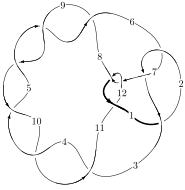
\includegraphics[width=112pt]{../../../GIT/diagram.site/Diagrams/png/1480_12a_0679.png}\\
\ \ \ A knot diagram\footnotemark}&
\allowdisplaybreaks
\textbf{Linearized knot diagam} \\
\cline{2-2}
 &
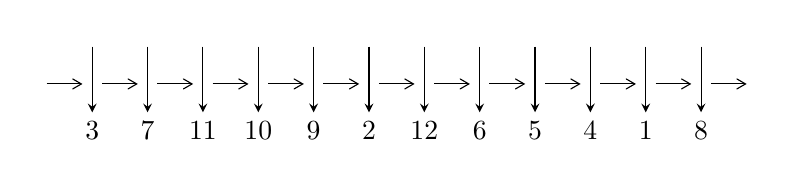
\begin{tikzpicture}[x=20pt, y=17pt]
	% nodes
	\node (C0) at (0, 0) {};
	\node (C1) at (1, 0) {};
	\node (C1U) at (1, +1) {};
	\node (C1D) at (1, -1) {3};

	\node (C2) at (2, 0) {};
	\node (C2U) at (2, +1) {};
	\node (C2D) at (2, -1) {7};

	\node (C3) at (3, 0) {};
	\node (C3U) at (3, +1) {};
	\node (C3D) at (3, -1) {11};

	\node (C4) at (4, 0) {};
	\node (C4U) at (4, +1) {};
	\node (C4D) at (4, -1) {10};

	\node (C5) at (5, 0) {};
	\node (C5U) at (5, +1) {};
	\node (C5D) at (5, -1) {9};

	\node (C6) at (6, 0) {};
	\node (C6U) at (6, +1) {};
	\node (C6D) at (6, -1) {2};

	\node (C7) at (7, 0) {};
	\node (C7U) at (7, +1) {};
	\node (C7D) at (7, -1) {12};

	\node (C8) at (8, 0) {};
	\node (C8U) at (8, +1) {};
	\node (C8D) at (8, -1) {6};

	\node (C9) at (9, 0) {};
	\node (C9U) at (9, +1) {};
	\node (C9D) at (9, -1) {5};

	\node (C10) at (10, 0) {};
	\node (C10U) at (10, +1) {};
	\node (C10D) at (10, -1) {4};

	\node (C11) at (11, 0) {};
	\node (C11U) at (11, +1) {};
	\node (C11D) at (11, -1) {1};

	\node (C12) at (12, 0) {};
	\node (C12U) at (12, +1) {};
	\node (C12D) at (12, -1) {8};
	\node (C13) at (13, 0) {};

	% arrows
	\draw[->,>={angle 60}]
	(C0) edge (C1) (C1) edge (C2) (C2) edge (C3) (C3) edge (C4) (C4) edge (C5) (C5) edge (C6) (C6) edge (C7) (C7) edge (C8) (C8) edge (C9) (C9) edge (C10) (C10) edge (C11) (C11) edge (C12) (C12) edge (C13) ;	\draw[->,>=stealth]
	(C1U) edge (C1D) (C2U) edge (C2D) (C3U) edge (C3D) (C4U) edge (C4D) (C5U) edge (C5D) (C6U) edge (C6D) (C7U) edge (C7D) (C8U) edge (C8D) (C9U) edge (C9D) (C10U) edge (C10D) (C11U) edge (C11D) (C12U) edge (C12D) ;
	\end{tikzpicture} \\
\hhline{~~} \\& 
\textbf{Solving Sequence} \\ \cline{2-2} 
 &
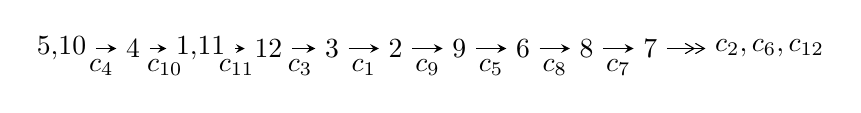
\begin{tikzpicture}[x=23pt, y=7pt]
	% node
	\node (A0) at (-1/8, 0) {5,10};
	\node (A1) at (1, 0) {4};
	\node (A2) at (33/16, 0) {1,11};
	\node (A3) at (25/8, 0) {12};
	\node (A4) at (33/8, 0) {3};
	\node (A5) at (41/8, 0) {2};
	\node (A6) at (49/8, 0) {9};
	\node (A7) at (57/8, 0) {6};
	\node (A8) at (65/8, 0) {8};
	\node (A9) at (73/8, 0) {7};
	\node (C1) at (1/2, -1) {$c_{4}$};
	\node (C2) at (3/2, -1) {$c_{10}$};
	\node (C3) at (21/8, -1) {$c_{11}$};
	\node (C4) at (29/8, -1) {$c_{3}$};
	\node (C5) at (37/8, -1) {$c_{1}$};
	\node (C6) at (45/8, -1) {$c_{9}$};
	\node (C7) at (53/8, -1) {$c_{5}$};
	\node (C8) at (61/8, -1) {$c_{8}$};
	\node (C9) at (69/8, -1) {$c_{7}$};
	\node (A10) at (11, 0) {$c_{2},c_{6},c_{12}$};

	% edge
	\draw[->,>=stealth]	
	(A0) edge (A1) (A1) edge (A2) (A2) edge (A3) (A3) edge (A4) (A4) edge (A5) (A5) edge (A6) (A6) edge (A7) (A7) edge (A8) (A8) edge (A9) ;
	\draw[->>,>={angle 60}]	
	(A9) edge (A10);
\end{tikzpicture} \\ 

\end{tabular} \\

\footnotetext{
The image of knot diagram is generated by the software ``\textbf{Draw programme}" developed by Andrew Bartholomew(\url{http://www.layer8.co.uk/maths/draw/index.htm\#Running-draw}), where we modified some parts for our purpose(\url{https://github.com/CATsTAILs/LinksPainter}).
}\phantom \\ \newline 
\centering \textbf{Ideals for irreducible components\footnotemark of $X_{\text{par}}$} 
 
\begin{align*}
I^u_{1}&=\langle 
u^{15}+2 u^{14}+\cdots+b-1,\;u^{18}+3 u^{17}+\cdots+2 a-4,\;u^{19}+3 u^{18}+\cdots-6 u-2\rangle \\
I^u_{2}&=\langle 
-7 u^{12} a+12 u^{12}+\cdots-4 a-9,\;u^{10} a+u^{11}+\cdots+a-1,\\
\phantom{I^u_{2}}&\phantom{= \langle  }u^{13}- u^{12}+10 u^{11}-9 u^{10}+37 u^9-29 u^8+62 u^7-40 u^6+46 u^5-22 u^4+12 u^3-3 u^2+u-1\rangle \\
I^u_{3}&=\langle 
b+u-2,\;3 a+2 u-3,\;u^2+3\rangle \\
I^u_{4}&=\langle 
b- u,\;a-1,\;u^2+1\rangle \\
\\
I^v_{1}&=\langle 
a,\;b+1,\;v+1\rangle \\
\end{align*}
\raggedright * 5 irreducible components of $\dim_{\mathbb{C}}=0$, with total 50 representations.\\
\footnotetext{All coefficients of polynomials are rational numbers. But the coefficients are sometimes approximated in decimal forms when there is not enough margin.}
\newpage
\renewcommand{\arraystretch}{1}
\centering \section*{I. $I^u_{1}= \langle u^{15}+2 u^{14}+\cdots+b-1,\;u^{18}+3 u^{17}+\cdots+2 a-4,\;u^{19}+3 u^{18}+\cdots-6 u-2 \rangle$}
\flushleft \textbf{(i) Arc colorings}\\
\begin{tabular}{m{7pt} m{180pt} m{7pt} m{180pt} }
\flushright $a_{5}=$&$\begin{pmatrix}1\\0\end{pmatrix}$ \\
\flushright $a_{10}=$&$\begin{pmatrix}0\\u\end{pmatrix}$ \\
\flushright $a_{4}=$&$\begin{pmatrix}1\\- u^2\end{pmatrix}$ \\
\flushright $a_{1}=$&$\begin{pmatrix}-\frac{1}{2} u^{18}-\frac{3}{2} u^{17}+\cdots+\frac{7}{2} u+2\\- u^{15}-2 u^{14}+\cdots+2 u+1\end{pmatrix}$ \\
\flushright $a_{11}=$&$\begin{pmatrix}- u\\u^3+u\end{pmatrix}$ \\
\flushright $a_{12}=$&$\begin{pmatrix}\frac{1}{2} u^{18}+\frac{3}{2} u^{17}+\cdots-\frac{9}{2} u-2\\u^{16}+2 u^{15}+\cdots- u-1\end{pmatrix}$ \\
\flushright $a_{3}=$&$\begin{pmatrix}u^2+1\\- u^4-2 u^2\end{pmatrix}$ \\
\flushright $a_{2}=$&$\begin{pmatrix}-\frac{1}{2} u^{18}-\frac{3}{2} u^{17}+\cdots+\frac{7}{2} u+1\\- u^{16}-2 u^{15}+\cdots+2 u+1\end{pmatrix}$ \\
\flushright $a_{9}=$&$\begin{pmatrix}u\\u\end{pmatrix}$ \\
\flushright $a_{6}=$&$\begin{pmatrix}u^2+1\\u^2\end{pmatrix}$ \\
\flushright $a_{8}=$&$\begin{pmatrix}u^3+2 u\\u^3+u\end{pmatrix}$ \\
\flushright $a_{7}=$&$\begin{pmatrix}\frac{1}{2} u^{18}+\frac{3}{2} u^{17}+\cdots-\frac{7}{2} u-1\\- u^{14}-2 u^{13}+\cdots+u+1\end{pmatrix}$\\&\end{tabular}
\flushleft \textbf{(ii) Obstruction class $= -1$}\\~\\
\flushleft \textbf{(iii) Cusp Shapes $= 2 u^{18}+6 u^{17}+36 u^{16}+86 u^{15}+264 u^{14}+506 u^{13}+1022 u^{12}+1566 u^{11}+2248 u^{10}+2704 u^9+2794 u^8+2526 u^7+1806 u^6+1106 u^5+464 u^4+122 u^3-16 u^2-28 u-20$}\\~\\
\newpage\renewcommand{\arraystretch}{1}
\flushleft \textbf{(iv) u-Polynomials at the component}\newline \\
\begin{tabular}{m{50pt}|m{274pt}}
Crossings & \hspace{64pt}u-Polynomials at each crossing \\
\hline $$\begin{aligned}c_{1},c_{11}\end{aligned}$$&$\begin{aligned}
&u^{19}+7 u^{18}+\cdots+13 u+1
\end{aligned}$\\
\hline $$\begin{aligned}c_{2},c_{6},c_{7}\\c_{12}\end{aligned}$$&$\begin{aligned}
&u^{19}- u^{18}+\cdots+u+1
\end{aligned}$\\
\hline $$\begin{aligned}c_{3},c_{4},c_{5}\\c_{8},c_{9},c_{10}\end{aligned}$$&$\begin{aligned}
&u^{19}-3 u^{18}+\cdots-6 u+2
\end{aligned}$\\
\hline
\end{tabular}\\~\\
\newpage\renewcommand{\arraystretch}{1}
\flushleft \textbf{(v) Riley Polynomials at the component}\newline \\
\begin{tabular}{m{50pt}|m{274pt}}
Crossings & \hspace{64pt}Riley Polynomials at each crossing \\
\hline $$\begin{aligned}c_{1},c_{11}\end{aligned}$$&$\begin{aligned}
&y^{19}+17 y^{18}+\cdots+37 y-1
\end{aligned}$\\
\hline $$\begin{aligned}c_{2},c_{6},c_{7}\\c_{12}\end{aligned}$$&$\begin{aligned}
&y^{19}-7 y^{18}+\cdots+13 y-1
\end{aligned}$\\
\hline $$\begin{aligned}c_{3},c_{4},c_{5}\\c_{8},c_{9},c_{10}\end{aligned}$$&$\begin{aligned}
&y^{19}+27 y^{18}+\cdots+24 y-4
\end{aligned}$\\
\hline
\end{tabular}\\~\\
\newpage\flushleft \textbf{(vi) Complex Volumes and Cusp Shapes}
$$\begin{array}{c|c|c}  
\text{Solutions to }I^u_{1}& \I (\text{vol} + \sqrt{-1}CS) & \text{Cusp shape}\\
 \hline 
\begin{aligned}
u &= -0.273151 + 0.815941 I \\
a &= -0.390307 - 0.220948 I \\
b &= -0.608791 + 0.652934 I\end{aligned}
 & \phantom{-}1.82620 - 1.77807 I & -6.92820 + 2.34039 I \\ \hline\begin{aligned}
u &= -0.273151 - 0.815941 I \\
a &= -0.390307 + 0.220948 I \\
b &= -0.608791 - 0.652934 I\end{aligned}
 & \phantom{-}1.82620 + 1.77807 I & -6.92820 - 2.34039 I \\ \hline\begin{aligned}
u &= \phantom{-}0.077265 + 0.786380 I \\
a &= -0.374812 - 0.399284 I \\
b &= -0.419169 + 0.348987 I\end{aligned}
 & \phantom{-}1.76915 - 1.42092 I & -5.09647 + 5.54292 I \\ \hline\begin{aligned}
u &= \phantom{-}0.077265 - 0.786380 I \\
a &= -0.374812 + 0.399284 I \\
b &= -0.419169 - 0.348987 I\end{aligned}
 & \phantom{-}1.76915 + 1.42092 I & -5.09647 - 5.54292 I \\ \hline\begin{aligned}
u &= -0.246012 + 1.236810 I \\
a &= -1.197950 + 0.527520 I \\
b &= \phantom{-}0.428066 - 0.067299 I\end{aligned}
 & \phantom{-}5.58686 + 10.56180 I & -7.44680 - 7.73425 I \\ \hline\begin{aligned}
u &= -0.246012 - 1.236810 I \\
a &= -1.197950 - 0.527520 I \\
b &= \phantom{-}0.428066 + 0.067299 I\end{aligned}
 & \phantom{-}5.58686 - 10.56180 I & -7.44680 + 7.73425 I \\ \hline\begin{aligned}
u &= -0.487418 + 0.522631 I \\
a &= \phantom{-}0.993393 - 0.218685 I \\
b &= \phantom{-}1.221660 + 0.201552 I\end{aligned}
 & -0.06851 + 8.01058 I & -10.52385 - 9.28102 I \\ \hline\begin{aligned}
u &= -0.487418 - 0.522631 I \\
a &= \phantom{-}0.993393 + 0.218685 I \\
b &= \phantom{-}1.221660 - 0.201552 I\end{aligned}
 & -0.06851 - 8.01058 I & -10.52385 + 9.28102 I \\ \hline\begin{aligned}
u &= -0.076466 + 1.310960 I \\
a &= \phantom{-}0.792972 - 0.747592 I \\
b &= -0.069397 - 0.530421 I\end{aligned}
 & \phantom{-}8.75335 - 0.83971 I & -3.29462 + 2.18721 I \\ \hline\begin{aligned}
u &= -0.076466 - 1.310960 I \\
a &= \phantom{-}0.792972 + 0.747592 I \\
b &= -0.069397 + 0.530421 I\end{aligned}
 & \phantom{-}8.75335 + 0.83971 I & -3.29462 - 2.18721 I\\
 \hline 
 \end{array}$$\newpage$$\begin{array}{c|c|c}  
\text{Solutions to }I^u_{1}& \I (\text{vol} + \sqrt{-1}CS) & \text{Cusp shape}\\
 \hline 
\begin{aligned}
u &= -0.550052 + 0.150551 I \\
a &= \phantom{-}0.41192 + 1.61654 I \\
b &= -0.276507 + 0.224858 I\end{aligned}
 & -1.18097 - 4.60134 I & -13.18408 + 3.99244 I \\ \hline\begin{aligned}
u &= -0.550052 - 0.150551 I \\
a &= \phantom{-}0.41192 - 1.61654 I \\
b &= -0.276507 - 0.224858 I\end{aligned}
 & -1.18097 + 4.60134 I & -13.18408 - 3.99244 I \\ \hline\begin{aligned}
u &= \phantom{-}0.308487\phantom{ +0.000000I} \\
a &= -0.641715\phantom{ +0.000000I} \\
b &= \phantom{-}0.245608\phantom{ +0.000000I}\end{aligned}
 & -0.592779\phantom{ +0.000000I} & -16.7390\phantom{ +0.000000I} \\ \hline\begin{aligned}
u &= -0.01455 + 1.70648 I \\
a &= -0.003380 - 1.097050 I \\
b &= -0.23251 - 1.76936 I\end{aligned}
 & \phantom{-}10.80000 - 1.26776 I & -5.99488 + 5.70666 I \\ \hline\begin{aligned}
u &= -0.01455 - 1.70648 I \\
a &= -0.003380 + 1.097050 I \\
b &= -0.23251 + 1.76936 I\end{aligned}
 & \phantom{-}10.80000 + 1.26776 I & -5.99488 - 5.70666 I \\ \hline\begin{aligned}
u &= -0.06366 + 1.79454 I \\
a &= -2.87448 + 0.37712 I \\
b &= -5.52313 + 0.65502 I\end{aligned}
 & \phantom{-}16.6584 + 11.9628 I & -6.98346 - 6.50856 I \\ \hline\begin{aligned}
u &= -0.06366 - 1.79454 I \\
a &= -2.87448 - 0.37712 I \\
b &= -5.52313 - 0.65502 I\end{aligned}
 & \phantom{-}16.6584 - 11.9628 I & -6.98346 + 6.50856 I \\ \hline\begin{aligned}
u &= -0.02020 + 1.81069 I \\
a &= \phantom{-}1.96350 - 0.53377 I \\
b &= \phantom{-}3.85697 - 1.33560 I\end{aligned}
 & -19.1741 - 0.3767 I & -3.17814 + 1.98776 I \\ \hline\begin{aligned}
u &= -0.02020 - 1.81069 I \\
a &= \phantom{-}1.96350 + 0.53377 I \\
b &= \phantom{-}3.85697 + 1.33560 I\end{aligned}
 & -19.1741 + 0.3767 I & -3.17814 - 1.98776 I\\
 \hline 
 \end{array}$$\newpage\newpage\renewcommand{\arraystretch}{1}
\centering \section*{II. $I^u_{2}= \langle -7 u^{12} a+12 u^{12}+\cdots-4 a-9,\;u^{10} a+u^{11}+\cdots+a-1,\;u^{13}- u^{12}+\cdots+u-1 \rangle$}
\flushleft \textbf{(i) Arc colorings}\\
\begin{tabular}{m{7pt} m{180pt} m{7pt} m{180pt} }
\flushright $a_{5}=$&$\begin{pmatrix}1\\0\end{pmatrix}$ \\
\flushright $a_{10}=$&$\begin{pmatrix}0\\u\end{pmatrix}$ \\
\flushright $a_{4}=$&$\begin{pmatrix}1\\- u^2\end{pmatrix}$ \\
\flushright $a_{1}=$&$\begin{pmatrix}a\\0.189189 a u^{12}-0.324324 u^{12}+\cdots+0.108108 a+0.243243\end{pmatrix}$ \\
\flushright $a_{11}=$&$\begin{pmatrix}- u\\u^3+u\end{pmatrix}$ \\
\flushright $a_{12}=$&$\begin{pmatrix}-0.567568 a u^{12}-0.0270270 u^{12}+\cdots+0.675676 a+0.270270\\-0.0810811 a u^{12}-0.432432 u^{12}+\cdots-0.189189 a+0.324324\end{pmatrix}$ \\
\flushright $a_{3}=$&$\begin{pmatrix}u^2+1\\- u^4-2 u^2\end{pmatrix}$ \\
\flushright $a_{2}=$&$\begin{pmatrix}0.108108 a u^{12}+0.243243 u^{12}+\cdots+0.918919 a-0.432432\\-0.0810811 a u^{12}-0.432432 u^{12}+\cdots-0.189189 a+0.324324\end{pmatrix}$ \\
\flushright $a_{9}=$&$\begin{pmatrix}u\\u\end{pmatrix}$ \\
\flushright $a_{6}=$&$\begin{pmatrix}u^2+1\\u^2\end{pmatrix}$ \\
\flushright $a_{8}=$&$\begin{pmatrix}u^3+2 u\\u^3+u\end{pmatrix}$ \\
\flushright $a_{7}=$&$\begin{pmatrix}-0.108108 a u^{12}-0.243243 u^{12}+\cdots-0.918919 a+0.432432\\u^{11}-2 u^{10}+\cdots+a u+u\end{pmatrix}$\\&\end{tabular}
\flushleft \textbf{(ii) Obstruction class $= -1$}\\~\\
\flushleft \textbf{(iii) Cusp Shapes $= -4 u^{11}+4 u^{10}-36 u^9+32 u^8-116 u^7+88 u^6-160 u^5+96 u^4-88 u^3+36 u^2-12 u-6$}\\~\\
\newpage\renewcommand{\arraystretch}{1}
\flushleft \textbf{(iv) u-Polynomials at the component}\newline \\
\begin{tabular}{m{50pt}|m{274pt}}
Crossings & \hspace{64pt}u-Polynomials at each crossing \\
\hline $$\begin{aligned}c_{1},c_{11}\end{aligned}$$&$\begin{aligned}
&u^{26}+13 u^{25}+\cdots+385 u+64
\end{aligned}$\\
\hline $$\begin{aligned}c_{2},c_{6},c_{7}\\c_{12}\end{aligned}$$&$\begin{aligned}
&u^{26}- u^{25}+\cdots-7 u+8
\end{aligned}$\\
\hline $$\begin{aligned}c_{3},c_{4},c_{5}\\c_{8},c_{9},c_{10}\end{aligned}$$&$\begin{aligned}
&(u^{13}+u^{12}+\cdots+u+1)^{2}
\end{aligned}$\\
\hline
\end{tabular}\\~\\
\newpage\renewcommand{\arraystretch}{1}
\flushleft \textbf{(v) Riley Polynomials at the component}\newline \\
\begin{tabular}{m{50pt}|m{274pt}}
Crossings & \hspace{64pt}Riley Polynomials at each crossing \\
\hline $$\begin{aligned}c_{1},c_{11}\end{aligned}$$&$\begin{aligned}
&y^{26}- y^{25}+\cdots+33151 y+4096
\end{aligned}$\\
\hline $$\begin{aligned}c_{2},c_{6},c_{7}\\c_{12}\end{aligned}$$&$\begin{aligned}
&y^{26}-13 y^{25}+\cdots-385 y+64
\end{aligned}$\\
\hline $$\begin{aligned}c_{3},c_{4},c_{5}\\c_{8},c_{9},c_{10}\end{aligned}$$&$\begin{aligned}
&(y^{13}+19 y^{12}+\cdots-5 y-1)^{2}
\end{aligned}$\\
\hline
\end{tabular}\\~\\
\newpage\flushleft \textbf{(vi) Complex Volumes and Cusp Shapes}
$$\begin{array}{c|c|c}  
\text{Solutions to }I^u_{2}& \I (\text{vol} + \sqrt{-1}CS) & \text{Cusp shape}\\
 \hline 
\begin{aligned}
u &= -0.083038 + 1.167020 I \\
a &= -0.182812 + 0.329365 I \\
b &= -0.28373 + 1.50091 I\end{aligned}
 & \phantom{-}1.55956 + 1.92579 I & -8.00122 - 3.82169 I \\ \hline\begin{aligned}
u &= -0.083038 + 1.167020 I \\
a &= -1.82248 - 0.57547 I \\
b &= \phantom{-}0.180439 - 0.168950 I\end{aligned}
 & \phantom{-}1.55956 + 1.92579 I & -8.00122 - 3.82169 I \\ \hline\begin{aligned}
u &= -0.083038 - 1.167020 I \\
a &= -0.182812 - 0.329365 I \\
b &= -0.28373 - 1.50091 I\end{aligned}
 & \phantom{-}1.55956 - 1.92579 I & -8.00122 + 3.82169 I \\ \hline\begin{aligned}
u &= -0.083038 - 1.167020 I \\
a &= -1.82248 + 0.57547 I \\
b &= \phantom{-}0.180439 + 0.168950 I\end{aligned}
 & \phantom{-}1.55956 - 1.92579 I & -8.00122 + 3.82169 I \\ \hline\begin{aligned}
u &= \phantom{-}0.179330 + 1.269600 I \\
a &= -0.753270 - 0.865498 I \\
b &= -0.137976 - 0.536137 I\end{aligned}
 & \phantom{-}7.63579 - 4.78537 I & -4.65540 + 3.59229 I \\ \hline\begin{aligned}
u &= \phantom{-}0.179330 + 1.269600 I \\
a &= \phantom{-}1.148590 + 0.147882 I \\
b &= -0.404842 - 0.185728 I\end{aligned}
 & \phantom{-}7.63579 - 4.78537 I & -4.65540 + 3.59229 I \\ \hline\begin{aligned}
u &= \phantom{-}0.179330 - 1.269600 I \\
a &= -0.753270 + 0.865498 I \\
b &= -0.137976 + 0.536137 I\end{aligned}
 & \phantom{-}7.63579 + 4.78537 I & -4.65540 - 3.59229 I \\ \hline\begin{aligned}
u &= \phantom{-}0.179330 - 1.269600 I \\
a &= \phantom{-}1.148590 - 0.147882 I \\
b &= -0.404842 + 0.185728 I\end{aligned}
 & \phantom{-}7.63579 + 4.78537 I & -4.65540 - 3.59229 I \\ \hline\begin{aligned}
u &= \phantom{-}0.379427 + 0.590112 I \\
a &= -0.841955 - 0.244681 I \\
b &= -1.020470 + 0.268374 I\end{aligned}
 & \phantom{-}1.59236 - 2.83275 I & -7.00318 + 5.17990 I \\ \hline\begin{aligned}
u &= \phantom{-}0.379427 + 0.590112 I \\
a &= \phantom{-}0.330450 - 0.407996 I \\
b &= \phantom{-}0.615126 + 0.383997 I\end{aligned}
 & \phantom{-}1.59236 - 2.83275 I & -7.00318 + 5.17990 I\\
 \hline 
 \end{array}$$\newpage$$\begin{array}{c|c|c}  
\text{Solutions to }I^u_{2}& \I (\text{vol} + \sqrt{-1}CS) & \text{Cusp shape}\\
 \hline 
\begin{aligned}
u &= \phantom{-}0.379427 - 0.590112 I \\
a &= -0.841955 + 0.244681 I \\
b &= -1.020470 - 0.268374 I\end{aligned}
 & \phantom{-}1.59236 + 2.83275 I & -7.00318 - 5.17990 I \\ \hline\begin{aligned}
u &= \phantom{-}0.379427 - 0.590112 I \\
a &= \phantom{-}0.330450 + 0.407996 I \\
b &= \phantom{-}0.615126 - 0.383997 I\end{aligned}
 & \phantom{-}1.59236 + 2.83275 I & -7.00318 - 5.17990 I \\ \hline\begin{aligned}
u &= \phantom{-}0.485085\phantom{ +0.000000I} \\
a &= -0.500820 + 1.088090 I \\
b &= \phantom{-}0.327558 + 0.106231 I\end{aligned}
 & -0.173769\phantom{ +0.000000I} & -11.9170\phantom{ +0.000000I} \\ \hline\begin{aligned}
u &= \phantom{-}0.485085\phantom{ +0.000000I} \\
a &= -0.500820 - 1.088090 I \\
b &= \phantom{-}0.327558 - 0.106231 I\end{aligned}
 & -0.173769\phantom{ +0.000000I} & -11.9170\phantom{ +0.000000I} \\ \hline\begin{aligned}
u &= -0.245118 + 0.346982 I \\
a &= \phantom{-}0.833919 + 0.205281 I \\
b &= \phantom{-}1.26442 + 0.90129 I\end{aligned}
 & -3.34890 + 0.88691 I & -13.3039 - 7.8258 I \\ \hline\begin{aligned}
u &= -0.245118 + 0.346982 I \\
a &= \phantom{-}0.69156 + 3.05215 I \\
b &= -0.067874 + 0.176233 I\end{aligned}
 & -3.34890 + 0.88691 I & -13.3039 - 7.8258 I \\ \hline\begin{aligned}
u &= -0.245118 - 0.346982 I \\
a &= \phantom{-}0.833919 - 0.205281 I \\
b &= \phantom{-}1.26442 - 0.90129 I\end{aligned}
 & -3.34890 - 0.88691 I & -13.3039 + 7.8258 I \\ \hline\begin{aligned}
u &= -0.245118 - 0.346982 I \\
a &= \phantom{-}0.69156 - 3.05215 I \\
b &= -0.067874 - 0.176233 I\end{aligned}
 & -3.34890 - 0.88691 I & -13.3039 + 7.8258 I \\ \hline\begin{aligned}
u &= -0.01838 + 1.78025 I \\
a &= \phantom{-}0.031468 - 1.234190 I \\
b &= -0.01017 - 1.63025 I\end{aligned}
 & \phantom{-}12.36340 + 2.35177 I & -7.64300 - 2.76650 I \\ \hline\begin{aligned}
u &= -0.01838 + 1.78025 I \\
a &= -3.09176 - 0.79285 I \\
b &= -6.07832 - 1.71326 I\end{aligned}
 & \phantom{-}12.36340 + 2.35177 I & -7.64300 - 2.76650 I\\
 \hline 
 \end{array}$$\newpage$$\begin{array}{c|c|c}  
\text{Solutions to }I^u_{2}& \I (\text{vol} + \sqrt{-1}CS) & \text{Cusp shape}\\
 \hline 
\begin{aligned}
u &= -0.01838 - 1.78025 I \\
a &= \phantom{-}0.031468 + 1.234190 I \\
b &= -0.01017 + 1.63025 I\end{aligned}
 & \phantom{-}12.36340 - 2.35177 I & -7.64300 + 2.76650 I \\ \hline\begin{aligned}
u &= -0.01838 - 1.78025 I \\
a &= -3.09176 + 0.79285 I \\
b &= -6.07832 + 1.71326 I\end{aligned}
 & \phantom{-}12.36340 - 2.35177 I & -7.64300 + 2.76650 I \\ \hline\begin{aligned}
u &= \phantom{-}0.04523 + 1.80316 I \\
a &= -1.62778 - 0.56147 I \\
b &= -3.25509 - 1.42971 I\end{aligned}
 & \phantom{-}18.9406 - 5.8171 I & -4.43476 + 2.75393 I \\ \hline\begin{aligned}
u &= \phantom{-}0.04523 + 1.80316 I \\
a &= \phantom{-}2.78489 + 0.06061 I \\
b &= \phantom{-}5.37092 - 0.01991 I\end{aligned}
 & \phantom{-}18.9406 - 5.8171 I & -4.43476 + 2.75393 I \\ \hline\begin{aligned}
u &= \phantom{-}0.04523 - 1.80316 I \\
a &= -1.62778 + 0.56147 I \\
b &= -3.25509 + 1.42971 I\end{aligned}
 & \phantom{-}18.9406 + 5.8171 I & -4.43476 - 2.75393 I \\ \hline\begin{aligned}
u &= \phantom{-}0.04523 - 1.80316 I \\
a &= \phantom{-}2.78489 - 0.06061 I \\
b &= \phantom{-}5.37092 + 0.01991 I\end{aligned}
 & \phantom{-}18.9406 + 5.8171 I & -4.43476 - 2.75393 I\\
 \hline 
 \end{array}$$\newpage\newpage\renewcommand{\arraystretch}{1}
\centering \section*{III. $I^u_{3}= \langle b+u-2,\;3 a+2 u-3,\;u^2+3 \rangle$}
\flushleft \textbf{(i) Arc colorings}\\
\begin{tabular}{m{7pt} m{180pt} m{7pt} m{180pt} }
\flushright $a_{5}=$&$\begin{pmatrix}1\\0\end{pmatrix}$ \\
\flushright $a_{10}=$&$\begin{pmatrix}0\\u\end{pmatrix}$ \\
\flushright $a_{4}=$&$\begin{pmatrix}1\\3\end{pmatrix}$ \\
\flushright $a_{1}=$&$\begin{pmatrix}-\frac{2}{3} u+1\\- u+2\end{pmatrix}$ \\
\flushright $a_{11}=$&$\begin{pmatrix}- u\\-2 u\end{pmatrix}$ \\
\flushright $a_{12}=$&$\begin{pmatrix}-\frac{5}{3} u+1\\-3 u+2\end{pmatrix}$ \\
\flushright $a_{3}=$&$\begin{pmatrix}-2\\-3\end{pmatrix}$ \\
\flushright $a_{2}=$&$\begin{pmatrix}-\frac{2}{3} u-1\\- u-1\end{pmatrix}$ \\
\flushright $a_{9}=$&$\begin{pmatrix}u\\u\end{pmatrix}$ \\
\flushright $a_{6}=$&$\begin{pmatrix}-2\\-3\end{pmatrix}$ \\
\flushright $a_{8}=$&$\begin{pmatrix}- u\\-2 u\end{pmatrix}$ \\
\flushright $a_{7}=$&$\begin{pmatrix}\frac{2}{3} u-1\\u-2\end{pmatrix}$\\&\end{tabular}
\flushleft \textbf{(ii) Obstruction class $= 1$}\\~\\
\flushleft \textbf{(iii) Cusp Shapes $= -12$}\\~\\
\newpage\renewcommand{\arraystretch}{1}
\flushleft \textbf{(iv) u-Polynomials at the component}\newline \\
\begin{tabular}{m{50pt}|m{274pt}}
Crossings & \hspace{64pt}u-Polynomials at each crossing \\
\hline $$\begin{aligned}c_{1},c_{2},c_{7}\\c_{11}\end{aligned}$$&$\begin{aligned}
&(u-1)^2
\end{aligned}$\\
\hline $$\begin{aligned}c_{3},c_{4},c_{5}\\c_{8},c_{9},c_{10}\end{aligned}$$&$\begin{aligned}
&u^2+3
\end{aligned}$\\
\hline $$\begin{aligned}c_{6},c_{12}\end{aligned}$$&$\begin{aligned}
&(u+1)^2
\end{aligned}$\\
\hline
\end{tabular}\\~\\
\newpage\renewcommand{\arraystretch}{1}
\flushleft \textbf{(v) Riley Polynomials at the component}\newline \\
\begin{tabular}{m{50pt}|m{274pt}}
Crossings & \hspace{64pt}Riley Polynomials at each crossing \\
\hline $$\begin{aligned}c_{1},c_{2},c_{6}\\c_{7},c_{11},c_{12}\end{aligned}$$&$\begin{aligned}
&(y-1)^2
\end{aligned}$\\
\hline $$\begin{aligned}c_{3},c_{4},c_{5}\\c_{8},c_{9},c_{10}\end{aligned}$$&$\begin{aligned}
&(y+3)^2
\end{aligned}$\\
\hline
\end{tabular}\\~\\
\newpage\flushleft \textbf{(vi) Complex Volumes and Cusp Shapes}
$$\begin{array}{c|c|c}  
\text{Solutions to }I^u_{3}& \I (\text{vol} + \sqrt{-1}CS) & \text{Cusp shape}\\
 \hline 
\begin{aligned}
u &= \phantom{-0.000000 -}1.73205 I \\
a &= \phantom{-}1.00000 - 1.15470 I \\
b &= \phantom{-}2.00000 - 1.73205 I\end{aligned}
 & \phantom{-}9.86960\phantom{ +0.000000I} & -12.0000\phantom{ +0.000000I} \\ \hline\begin{aligned}
u &= \phantom{-0.000000 } -1.73205 I \\
a &= \phantom{-}1.00000 + 1.15470 I \\
b &= \phantom{-}2.00000 + 1.73205 I\end{aligned}
 & \phantom{-}9.86960\phantom{ +0.000000I} & -12.0000\phantom{ +0.000000I}\\
 \hline 
 \end{array}$$\newpage\newpage\renewcommand{\arraystretch}{1}
\centering \section*{IV. $I^u_{4}= \langle b- u,\;a-1,\;u^2+1 \rangle$}
\flushleft \textbf{(i) Arc colorings}\\
\begin{tabular}{m{7pt} m{180pt} m{7pt} m{180pt} }
\flushright $a_{5}=$&$\begin{pmatrix}1\\0\end{pmatrix}$ \\
\flushright $a_{10}=$&$\begin{pmatrix}0\\u\end{pmatrix}$ \\
\flushright $a_{4}=$&$\begin{pmatrix}1\\1\end{pmatrix}$ \\
\flushright $a_{1}=$&$\begin{pmatrix}1\\u\end{pmatrix}$ \\
\flushright $a_{11}=$&$\begin{pmatrix}- u\\0\end{pmatrix}$ \\
\flushright $a_{12}=$&$\begin{pmatrix}- u+1\\u\end{pmatrix}$ \\
\flushright $a_{3}=$&$\begin{pmatrix}0\\1\end{pmatrix}$ \\
\flushright $a_{2}=$&$\begin{pmatrix}1\\u+1\end{pmatrix}$ \\
\flushright $a_{9}=$&$\begin{pmatrix}u\\u\end{pmatrix}$ \\
\flushright $a_{6}=$&$\begin{pmatrix}0\\-1\end{pmatrix}$ \\
\flushright $a_{8}=$&$\begin{pmatrix}u\\0\end{pmatrix}$ \\
\flushright $a_{7}=$&$\begin{pmatrix}1\\u\end{pmatrix}$\\&\end{tabular}
\flushleft \textbf{(ii) Obstruction class $= 1$}\\~\\
\flushleft \textbf{(iii) Cusp Shapes $= -12$}\\~\\
\newpage\renewcommand{\arraystretch}{1}
\flushleft \textbf{(iv) u-Polynomials at the component}\newline \\
\begin{tabular}{m{50pt}|m{274pt}}
Crossings & \hspace{64pt}u-Polynomials at each crossing \\
\hline $$\begin{aligned}c_{1},c_{6},c_{11}\\c_{12}\end{aligned}$$&$\begin{aligned}
&(u-1)^2
\end{aligned}$\\
\hline $$\begin{aligned}c_{2},c_{7}\end{aligned}$$&$\begin{aligned}
&(u+1)^2
\end{aligned}$\\
\hline $$\begin{aligned}c_{3},c_{4},c_{5}\\c_{8},c_{9},c_{10}\end{aligned}$$&$\begin{aligned}
&u^2+1
\end{aligned}$\\
\hline
\end{tabular}\\~\\
\newpage\renewcommand{\arraystretch}{1}
\flushleft \textbf{(v) Riley Polynomials at the component}\newline \\
\begin{tabular}{m{50pt}|m{274pt}}
Crossings & \hspace{64pt}Riley Polynomials at each crossing \\
\hline $$\begin{aligned}c_{1},c_{2},c_{6}\\c_{7},c_{11},c_{12}\end{aligned}$$&$\begin{aligned}
&(y-1)^2
\end{aligned}$\\
\hline $$\begin{aligned}c_{3},c_{4},c_{5}\\c_{8},c_{9},c_{10}\end{aligned}$$&$\begin{aligned}
&(y+1)^2
\end{aligned}$\\
\hline
\end{tabular}\\~\\
\newpage\flushleft \textbf{(vi) Complex Volumes and Cusp Shapes}
$$\begin{array}{c|c|c}  
\text{Solutions to }I^u_{4}& \I (\text{vol} + \sqrt{-1}CS) & \text{Cusp shape}\\
 \hline 
\begin{aligned}
u &= \phantom{-0.000000 -}1.000000 I \\
a &= \phantom{-}1.00000\phantom{ +0.000000I} \\
b &= \phantom{-0.000000 -}1.000000 I\end{aligned}
 & \phantom{-0.000000 } 0 & -12.0000\phantom{ +0.000000I} \\ \hline\begin{aligned}
u &= \phantom{-0.000000 } -1.000000 I \\
a &= \phantom{-}1.00000\phantom{ +0.000000I} \\
b &= \phantom{-0.000000 } -1.000000 I\end{aligned}
 & \phantom{-0.000000 } 0 & -12.0000\phantom{ +0.000000I}\\
 \hline 
 \end{array}$$\newpage\newpage\renewcommand{\arraystretch}{1}
\centering \section*{V. $I^v_{1}= \langle a,\;b+1,\;v+1 \rangle$}
\flushleft \textbf{(i) Arc colorings}\\
\begin{tabular}{m{7pt} m{180pt} m{7pt} m{180pt} }
\flushright $a_{5}=$&$\begin{pmatrix}1\\0\end{pmatrix}$ \\
\flushright $a_{10}=$&$\begin{pmatrix}-1\\0\end{pmatrix}$ \\
\flushright $a_{4}=$&$\begin{pmatrix}1\\0\end{pmatrix}$ \\
\flushright $a_{1}=$&$\begin{pmatrix}0\\-1\end{pmatrix}$ \\
\flushright $a_{11}=$&$\begin{pmatrix}-1\\0\end{pmatrix}$ \\
\flushright $a_{12}=$&$\begin{pmatrix}-1\\-1\end{pmatrix}$ \\
\flushright $a_{3}=$&$\begin{pmatrix}1\\0\end{pmatrix}$ \\
\flushright $a_{2}=$&$\begin{pmatrix}1\\-1\end{pmatrix}$ \\
\flushright $a_{9}=$&$\begin{pmatrix}-1\\0\end{pmatrix}$ \\
\flushright $a_{6}=$&$\begin{pmatrix}1\\0\end{pmatrix}$ \\
\flushright $a_{8}=$&$\begin{pmatrix}-1\\0\end{pmatrix}$ \\
\flushright $a_{7}=$&$\begin{pmatrix}0\\1\end{pmatrix}$\\&\end{tabular}
\flushleft \textbf{(ii) Obstruction class $= 1$}\\~\\
\flushleft \textbf{(iii) Cusp Shapes $= -12$}\\~\\
\newpage\renewcommand{\arraystretch}{1}
\flushleft \textbf{(iv) u-Polynomials at the component}\newline \\
\begin{tabular}{m{50pt}|m{274pt}}
Crossings & \hspace{64pt}u-Polynomials at each crossing \\
\hline $$\begin{aligned}c_{1},c_{2},c_{7}\\c_{11}\end{aligned}$$&$\begin{aligned}
&u-1
\end{aligned}$\\
\hline $$\begin{aligned}c_{3},c_{4},c_{5}\\c_{8},c_{9},c_{10}\end{aligned}$$&$\begin{aligned}
&u
\end{aligned}$\\
\hline $$\begin{aligned}c_{6},c_{12}\end{aligned}$$&$\begin{aligned}
&u+1
\end{aligned}$\\
\hline
\end{tabular}\\~\\
\newpage\renewcommand{\arraystretch}{1}
\flushleft \textbf{(v) Riley Polynomials at the component}\newline \\
\begin{tabular}{m{50pt}|m{274pt}}
Crossings & \hspace{64pt}Riley Polynomials at each crossing \\
\hline $$\begin{aligned}c_{1},c_{2},c_{6}\\c_{7},c_{11},c_{12}\end{aligned}$$&$\begin{aligned}
&y-1
\end{aligned}$\\
\hline $$\begin{aligned}c_{3},c_{4},c_{5}\\c_{8},c_{9},c_{10}\end{aligned}$$&$\begin{aligned}
&y
\end{aligned}$\\
\hline
\end{tabular}\\~\\
\newpage\flushleft \textbf{(vi) Complex Volumes and Cusp Shapes}
$$\begin{array}{c|c|c}  
\text{Solutions to }I^v_{1}& \I (\text{vol} + \sqrt{-1}CS) & \text{Cusp shape}\\
 \hline 
\begin{aligned}
v &= -1.00000\phantom{ +0.000000I} \\
a &= \phantom{-0.000000 } 0 \\
b &= -1.00000\phantom{ +0.000000I}\end{aligned}
 & -3.28987\phantom{ +0.000000I} & -12.0000\phantom{ +0.000000I}\\
 \hline 
 \end{array}$$\newpage
\newpage\renewcommand{\arraystretch}{1}
\centering \section*{ VI. u-Polynomials}
\begin{tabular}{m{50pt}|m{274pt}}
Crossings & \hspace{64pt}u-Polynomials at each crossing \\
\hline $$\begin{aligned}c_{1},c_{11}\end{aligned}$$&$\begin{aligned}
&((u-1)^5)(u^{19}+7 u^{18}+\cdots+13 u+1)(u^{26}+13 u^{25}+\cdots+385 u+64)
\end{aligned}$\\
\hline $$\begin{aligned}c_{2},c_{7}\end{aligned}$$&$\begin{aligned}
&((u-1)^3)(u+1)^2(u^{19}- u^{18}+\cdots+u+1)(u^{26}- u^{25}+\cdots-7 u+8)
\end{aligned}$\\
\hline $$\begin{aligned}c_{3},c_{4},c_{5}\\c_{8},c_{9},c_{10}\end{aligned}$$&$\begin{aligned}
&u(u^2+1)(u^2+3)(u^{13}+u^{12}+\cdots+u+1)^{2}(u^{19}-3 u^{18}+\cdots-6 u+2)
\end{aligned}$\\
\hline $$\begin{aligned}c_{6},c_{12}\end{aligned}$$&$\begin{aligned}
&((u-1)^2)(u+1)^3(u^{19}- u^{18}+\cdots+u+1)(u^{26}- u^{25}+\cdots-7 u+8)
\end{aligned}$\\
\hline
\end{tabular}\newpage\renewcommand{\arraystretch}{1}
\centering \section*{ VII. Riley Polynomials}
\begin{tabular}{m{50pt}|m{274pt}}
Crossings & \hspace{64pt}Riley Polynomials at each crossing \\
\hline $$\begin{aligned}c_{1},c_{11}\end{aligned}$$&$\begin{aligned}
&((y-1)^5)(y^{19}+17 y^{18}+\cdots+37 y-1)\\
&\cdot(y^{26}- y^{25}+\cdots+33151 y+4096)
\end{aligned}$\\
\hline $$\begin{aligned}c_{2},c_{6},c_{7}\\c_{12}\end{aligned}$$&$\begin{aligned}
&((y-1)^5)(y^{19}-7 y^{18}+\cdots+13 y-1)(y^{26}-13 y^{25}+\cdots-385 y+64)
\end{aligned}$\\
\hline $$\begin{aligned}c_{3},c_{4},c_{5}\\c_{8},c_{9},c_{10}\end{aligned}$$&$\begin{aligned}
&y(y+1)^2(y+3)^2(y^{13}+19 y^{12}+\cdots-5 y-1)^{2}\\
&\cdot(y^{19}+27 y^{18}+\cdots+24 y-4)
\end{aligned}$\\
\hline
\end{tabular}
\vskip 2pc
\end{document}